\documentclass{article}
\usepackage[utf8]{inputenc}

% Preamble
\usepackage{amsmath}
\usepackage[margin=3cm, top=2cm, bottom=2cm]{geometry}
\usepackage{parskip}
   \setlength{\parindent}{0pt} % No automatic indent
\usepackage{setspace}
   \onehalfspacing
\usepackage{graphicx}
\usepackage{enumitem} % Lists
\usepackage{tabularx} % Tables
\usepackage{amssymb}  % For real numbers
\usepackage{dsfont}   % Indicator function (mathds{1})
%\usepackage[backend=bibtex]{biblatex}
\usepackage[round]{natbib}
\bibliographystyle{plainnat}
%\bibliography{bibliography}
\usepackage{placeins}
\usepackage{caption}

\usepackage{etoolbox}
\usepackage{float}  % Figure H placement
\patchcmd{\thebibliography}{\chapter*}{\section*}{}{} % Bibliography in same page
\usepackage{url}    % URL modes
%\decimalpoint % Point instead of comma for decimal places
\usepackage{hyperref}
%\usepackage{caption}
%\usepackage{subcaption}
\usepackage{wrapfig}
\usepackage[usenames, dvipsnames]{color}

% Aside environment definition
\usepackage{mdframed}
\newenvironment{aside}
  {\begin{mdframed}[style=0,%
      leftline=false,rightline=false,leftmargin=2em,rightmargin=2em,%
          innerleftmargin=0pt,innerrightmargin=0pt,linewidth=0.75pt,%
      skipabove=7pt,skipbelow=7pt]\small}
  {\end{mdframed}}


%\usepackage{xcolor}
\usepackage[normalem]{ulem}
\useunder{\uline}{\ulined}{}%
\DeclareUrlCommand{\bulurl}{\def\UrlFont{\ttfamily\color{blue}\ulined}}


\begin{document}


\title{\vspace{-1.2cm}Text Mining the Sentiments Behind the Grammys}
\author{Gian Carlo Di-Luvi \\
{\normalsize Business Analytics Coordinator at Pfizer Inc.} \\
{\normalsize E-mail address: \href{mailto:giancarlo.diluvi@pfizer.com}{GianCarlo.Diluvi@pfizer.com}}}
\date{}

\maketitle


Music permeates our life as one of the foremost forms of human expression. From our everyday activities to the most important moments in life, music is a part of it all and, thus, there have been many attempts to quantify it in one way or another. Of the many aspects of music, lyrics are of particular relevance because most contemporary artists impose their intended message within them. It is then possible to draw meaningful conclusions from a song by analyzing its lyrics. In this paper, I use text mining and sentiment analysis to look at statistical aspects of lyrics of popular songs from 1960 onwards.



%Music permeates our life as one of the foremost forms of human expression. From our everyday activities to the most important moments in life, music is a part of it all. Like other art forms, music often reflects the world's overall state of affairs and, thus, there have been many attempts to quantify it in one way or another. Of the many aspects of music, lyrics are of particular relevance because most contemporary artists impose their intended message within them. It is then possible to draw meaningful conclusions from a song---and its reflection of the state of the world---by analyzing its lyrics. In this paper, I use text mining and sentiment analysis to look at statistical aspects of lyrics of popular songs from 1960 onwards.

%Moreover, the entertainment industry is one of the biggest in the world, accounting for \hyperref[https://www.statista.com/statistics/237749/value-of-the-global-entertainment-and-media-market/]{more than \$1.5 trillion USD in 2015}. \\


%Of the many aspects of music, lyrics are of particular relevance because most contemporary artists impose their intended message within them. Thus, it is possible to draw meaningful conclusions of a song by analyzing its lyrics.  \\







\section*{Quantifying music}


Objectively studying music is a difficult task at best. Ideally, one would have to analyze all the music released on a given year or years, all around the world. One way to simplify this problem is narrowing down the analysis to only those musical creations that have been held as exceptional. Thankfully, a large number of musical awards are constantly given to artists, producers, composers, and all people involved in the music-making process. These highlight and recognize precisely those musicians that have created outstanding musical pieces. With this in mind, I narrowed down the analysis to winners of one particular award: The Grammy Award for Album of the Year.  \\


The Grammy Awards, named in honor of the gramophone, are arguably one of the most famous and prestigious musical awards. They originated in the late 1950's, when music executives decided to create an award equivalent to the Academy Awards (for film) and the Emmy Awards (for television). Since 1959, Grammy Awards are given every year by The Recording Academy for different categories, such as Record of the Year, Song of the Year, Best New Artist, and Album of the Year. The last one is of special interest because it is awarded based on the quality of the album as a whole, and not on the merit of individual songs. \\


%Text mining techniques can be applied to texts from different origins, such as political speeches, novels or, yes, song lyrics. With it, different texts can be objectively compared. \\

For this analysis, and with the help of the \texttt{genius} package in \textsf{R} (Parry, 2018), I obtained from \href{https://genius.com/}{\bulurl{Genius}}, an online song lyrics repository, the lyrics in English of all the songs of each album that won the Grammy Award for Album of the Year from 1960 to 2019. It should be mentioned that four albums, all from the 60's, were omitted from the analysis: Bob Newhart's 1961 \textit{The Button-Down Mind of Bob Newhart} and Vaughn Meader's 1963 \textit{The First Family} are comedy albums; Judy Garland's 1962 \textit{Judy at Carnegie Hall} is a live album; and Stan Getz and Jo\~{a}o Gilberto's 1964 \textit{Getz/Gilberto} has lyrics in Portuguese.  \\

%Henry Mancini's 1959 \textit{The Music from Peter Gunn} is instrumental; 

%\begin{wrapfigure}{l}{0.6\textwidth}
%    \centering
%    \includegraphics[width=0.55\textwidth]{graph_common_words.pdf}
%    \caption{The ten most common words of the songs of all the albums that won the Grammy Award for Album of the Year are shown, along with the number of times they appear.}
%    \label{fig:common_words}
%\end{wrapfigure}

%As time passes, not only do bigger amounts of data become easier to access, but also in much more different forms. As such, it is of interest to develop techniques that allow us to analyze this ever-growing data heterogeneity. \textit{Text mining} is but one such set of techniques, whose purpose is to process, transform, and study information in the form of text so that statistical conclusions can be derived from it. \\


After joining the lyrics of the 56 albums---comprising 761 songs---in a single data set, it was possible to start analyzing the data via \textit{text mining}, a set of techniques whose purpose is to process, transform, and study information in the form of text so that statistical conclusions can be derived from it. For instance, the average number of songs per album throughout this period is around 13.5, with the 80s having a low 11.5 and the 2000s having the largest at more than 16 (mainly due to Outkast's 2003 \textit{Speakerboxxx/The Love Below}, which featured 40 songs). \\

%\newpage

There are exactly 185,091 words in my data set, averaging around 240 per song. The 60s are by far the decade with the lowest average word count per song, with 161, versus the much higher 297 from 2010 to 2019. Figure \ref{fig:boxplot_WpS} shows how there seems to be a slight increase in the number of words per song over time. \\

Figure \ref{fig:common_words} shows the ten most common words in all those songs, without taking into account the usual English stop words such as `the', `of', `to', etc. (Stop words can easily be removed from a tidy data set with the \texttt{tidytext} \textsf{R} package \citep{text_mining_r}.)

\begin{figure}[h]
    \centering
    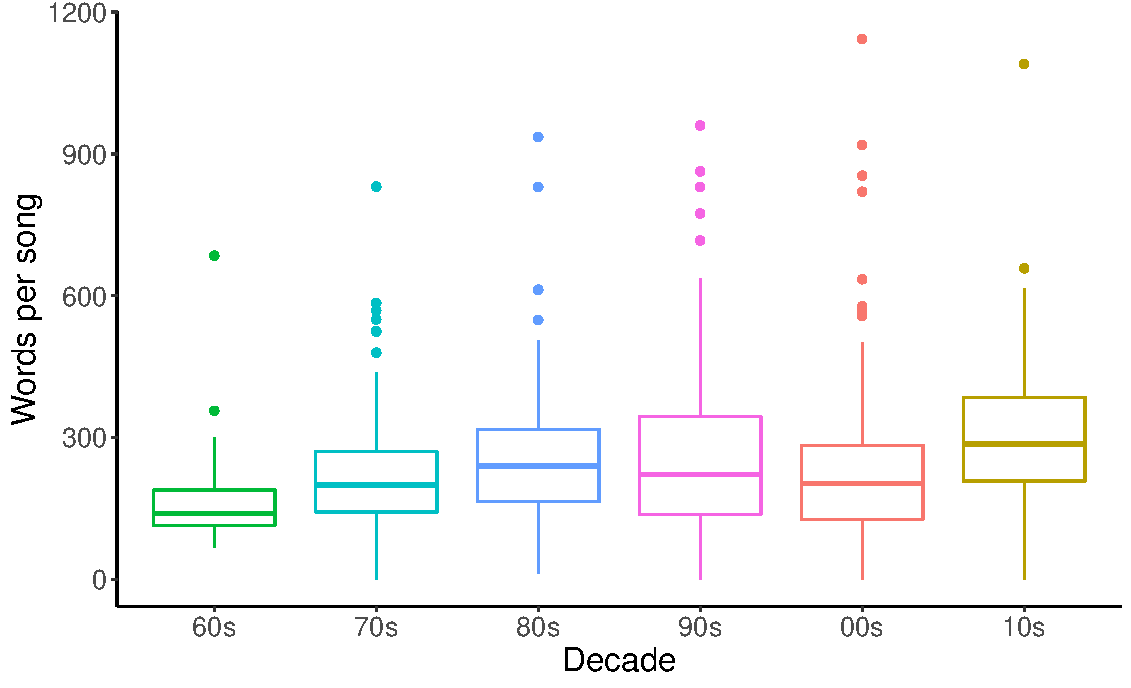
\includegraphics[scale=0.5]{Plots/Boxplot_WpS.pdf}
    \caption{Boxplot of the number of words per song by decade of the Grammy Albums of the Year, 1960--2019.}
    \label{fig:boxplot_WpS}
\end{figure}





\begin{figure}[h]
    \centering
    \includegraphics[scale=0.5]{Plots/graph_common_words.pdf}
    \caption{The ten most common words of the songs of all the Grammy Albums of the Year, 1960--2019.}
    \label{fig:common_words}
\end{figure}

%\newpage

Amusingly, although perhaps not surprisingly, `love' is the most common word across all songs. Moreover, this is also true if one looks at each individual decade, as can be seen in Figure \ref{fig:common_words_decade}. This last Figure also shows that `baby' has been the second most popular word for the past three decades.


% na: Paul Simon's Diamond on the Soles of her Shows (unreleased version)
% ey: Taylor Swift's Wonderland
% la: The Boxer and Another Star
% ih: Homeless (Ft. Joseph Shabalala & Ladysmith Black Mambazo)

\begin{figure}[h]
    \centering
    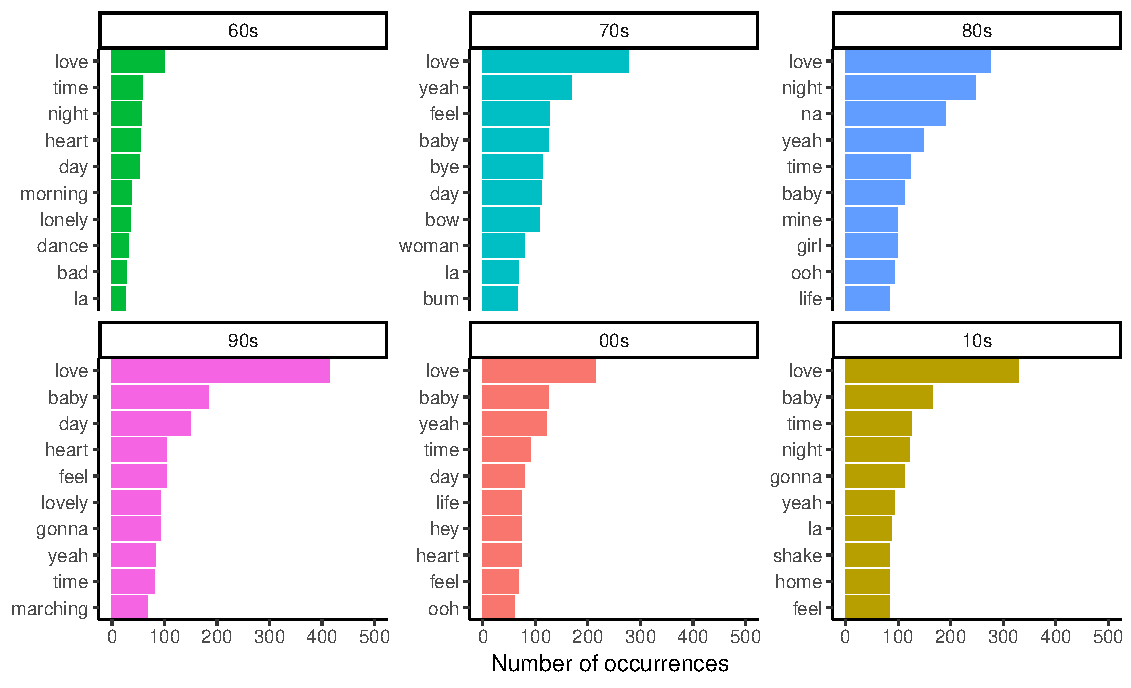
\includegraphics[scale=0.65]{Plots/graph_common_words_decade_FW.pdf}
    \caption{The ten most common words of the songs of all the Grammy Albums of the Year, 1960--2019, by decade.}
    \label{fig:common_words_decade}
\end{figure}


\FloatBarrier


\begin{aside}
        Something interesting in Figure \ref{fig:common_words_decade} is the appearance of rather odd words in some decades. For example, the popularity of the word `la' in the 60s is due to Barbra Streisand's 1964 interpretation of ``Who's Afraid of the Big Bad Wolf'' (``...who's afraid of the big bad wolf / tra la la la la...''); in the 70s it mostly appears in Simon and Garfunkel's 1971 ``The Boxer'' and in the 10s its popularity is due to ``Deep Blue'' by Arcade Fire. The word `na' appears more than 100 times in the unreleased version of Paul Simon's 1987 ``Diamonds on the Soles of Her Shoes,'' and more than 30 times in the same album's ``You Can Call Me Al,'' as well as in Michael Jackson's 1984 ``P.Y.T. (Pretty Young Thing),'' making it the third most common word of the 80s. Similarly, `bum' appears on the chorus of Stevie Wonder's 1975 ``Smile Please'' (``Bum, bum bum ditti / Bum, bum bum ditti...''). Finally, `ooh' appears a large amount of times in both OutKast's 2004 ``Roses'' (``Roses really smell like poo-ooh-ooh...'') and in the chorus of U2's 2006 ``City of Blinding Lights.'' (It can, of course, be argued that none of this expressions are real words.)
\end{aside}

%That same decade the tenth most common word was `ih', which refers to the gasping sounds of Paul Simon's 1987 ``Homeless.''



%\FloatBarrier
\section*{The sentiments of sentimentality}


Just by looking at the most common words by decade, it is possible to try to guess which decades were, say, happier than others. For example, `lonely' and `bad' (words with a negative connotation) were prominent words in the 60s, whereas `baby', `heart', `lovely', and `yeah' (words with a more positive connotation) were more common in the 90s. This may lead us to hypothesize that the 90s had a lighter mood than the 60s. \\


The reasoning behind that example is the basis for \textit{sentiment analysis}, a series of techniques that help quantify emotions or affective states. Human writing is necessarily loaded with emotional intent in its words, and part of successful reading is the correct interpretation of those sentiments. Sentiment analysis aims to reproduce this mental process programmatically, using objective methods (without forgetting that, in the end, what is being studied is subjective by nature). \\


%\newpage

There exist a variety of ways of doing this. The most popular ones rely on assigning sentiments to individual words, and then obtaining the net sentiment of a text by adding up the sentiments of the words that make it up. These so-called vocabulary lexicons contain a large number of English words with their respective sentiment (or sentiments) and are usually obtained and verified by hand. \\




For this analysis I used the \cite{Liu_sentiments} lexicon, which categorizes words as either `positive' or `negative' in a binary fashion. A `positive' and a `negative' score are computed by counting the number of words within each category, and the net sentiment is obtained by subtracting the latter from the former. Liu's lexicon can be found in the \texttt{sentiments} data set from the \texttt{tidytext} \textsf{R} package. \\


It is worth noting some implications of this approach. First, many English words are omitted from Liu's lexicon because they are relatively neutral, which makes it difficult to assign a sentiment to them. Second, one may also argue that there exist multiple levels of positive and negative connotations, that is, not all positive words are equally positive. Although other lexicons do take this fact into account, it may also be argued that, if Liu's lexicon is subjective as it is, adding more levels will only increase that subjectivity. Thus, using another lexicon does not bring enough benefits to have a dramatic impact on the quality of the analysis. All in all, lexicon-based sentiment analysis offers an easy approach to analyzing emotions in text, although its limitations must be considered. \\



With that in mind, I applied Liu's lexicon to every song in the data set to generate a net sentiment score by album, which is shown in Figure \ref{fig:annual_sentiment}. From this graph we can see that the three albums with the greatest net sentiment belong to the 90s: Whitney Houston's 1994 \textit{The Bodyguard: Original Soundtrack Album}, Natalie Cole's 1992 \textit{Unforgettable... with Love}, and Celine Dion's 1997 \textit{Falling into You}, respectively. Moreover, the 90s are the only decade in which no album has a negative net sentiment score. The 2010s are also an interesting decade in that they have the album with the fourth highest net sentiment (Bruno Mars' 2018 \textit{24K Magic}), and also the one with the lowest one (Mumford \& Sons' 2013 \textit{Babel}).


\begin{figure}[h]
    \centering
    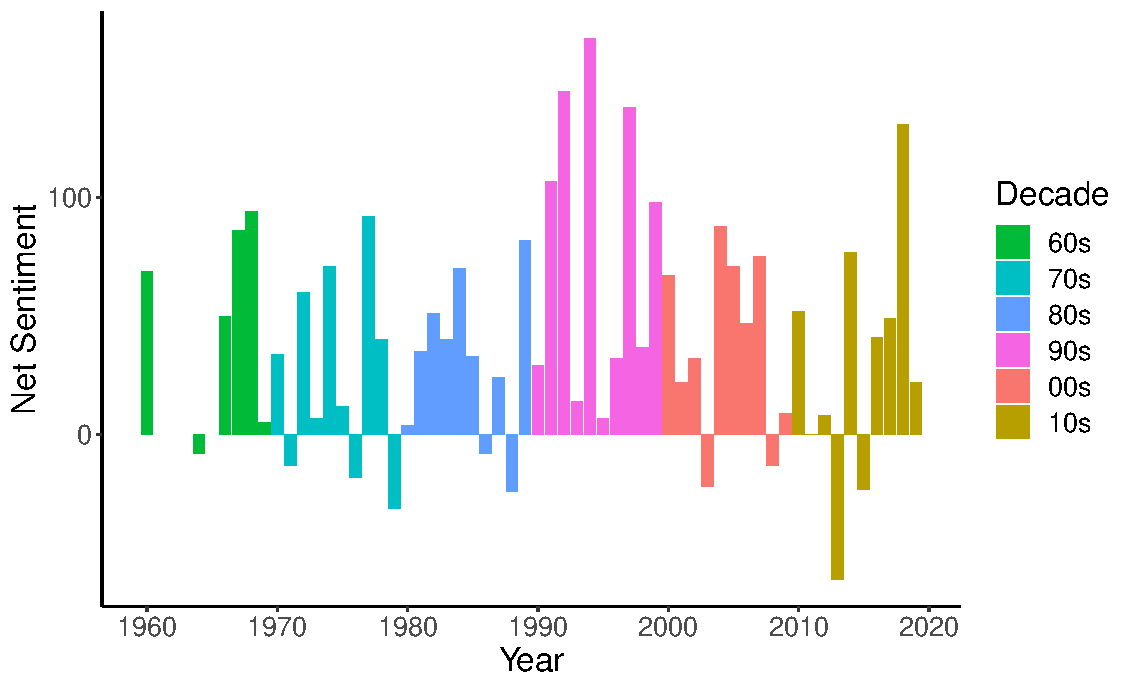
\includegraphics[scale=0.5]{Plots/graph_annual_sentiment.pdf}
    \caption{Net sentiment scores of the Grammy Albums of the Year, 1960--2019. Missing values in the 60s correspond to the 4 albums omitted from the analysis.}
    \label{fig:annual_sentiment}
\end{figure}


%\begin{wrapfigure}{r}{0.6\textwidth}
%    \centering
%    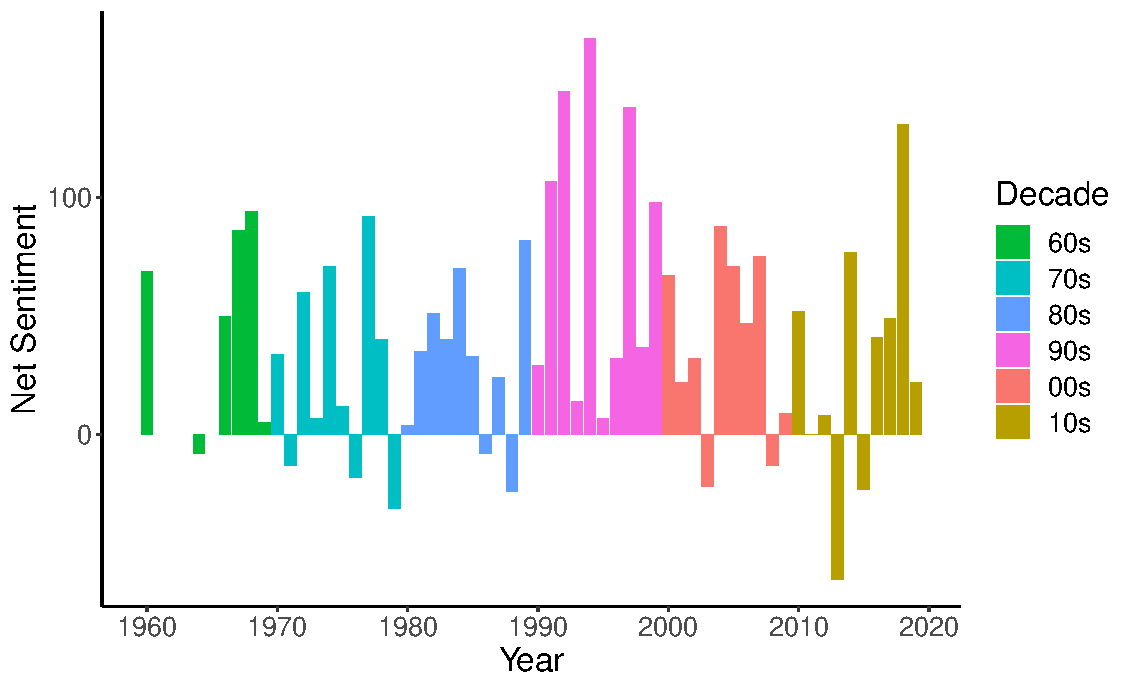
\includegraphics[width=0.55\textwidth]{Plots/graph_annual_sentiment.pdf}
%    \caption{Net sentiment scores by album, using color to differentiate between decades. Missing values correspond to the 4 albums omitted from the analysis.}
%    \label{fig:annual_sentiment}
%\end{wrapfigure}


%One could then try to predict what the net sentiment of future winners of the Grammy Award will be. 

One could then try to study the evolution of the Grammy Albums of the Year's net sentiments over time. One way to do this is by explaining the relationship between the year and the net sentiment with a \textit{linear regression}. This model associates the net sentiment of an album that won the Grammy Award with the year it was released via a linear equation, that is,
\begin{equation*}
    \text{Net sentiment} = a + b \times \text{year},
\end{equation*}
where both $a$ and $b$ are unknown parameters to be estimated with the information of the albums that have won in previous years. The parameter $b$ quantifies how much the net sentiment changes from one year to the next, and it has to be statistically different from zero for the model to be significant. However, the estimated value obtained from the data ($\hat{b} = 0.022$) could not be determined to be different from zero. Figure \ref{fig:sentiment_lm} shows the data points with the estimated linear equation in red, where it is clear that there does not seem to be any meaningful relationship between the net sentiment and the year. This means that the net sentiment of Grammy Award winners, although certainly higher or lower some years, has remained relatively stable overall.  


\begin{figure}[h]
    \centering
    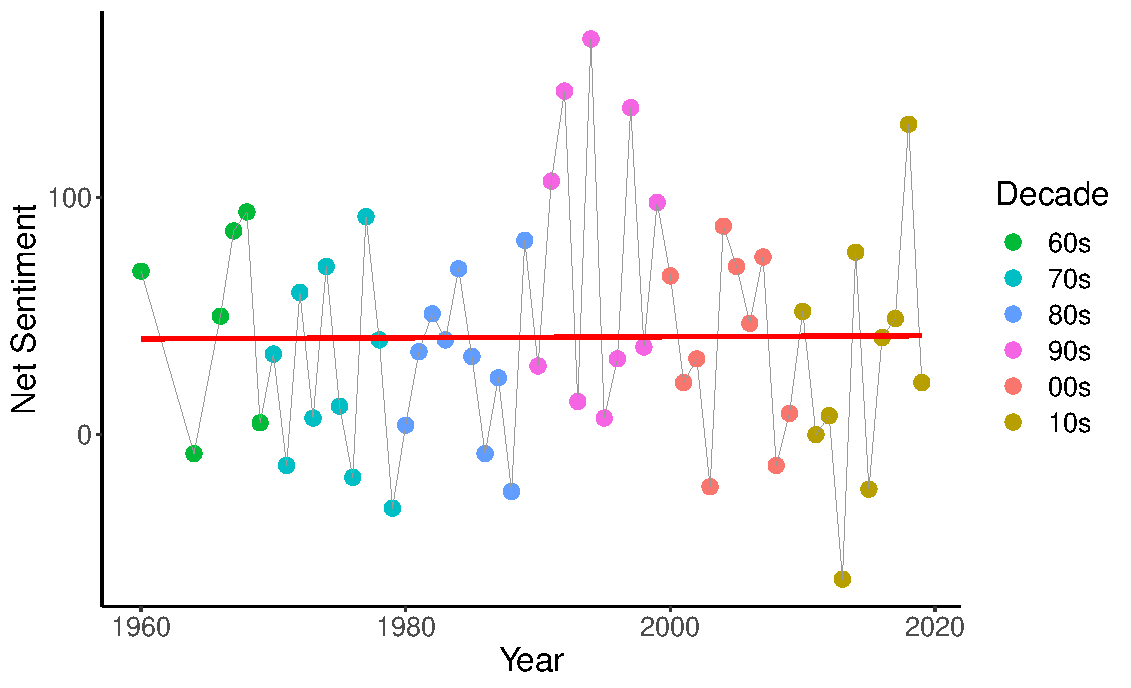
\includegraphics[scale=0.5]{Plots/graph_sentiment_linear_trend.pdf}
    \caption{Net sentiment of the Grammy Albums of the Year, 1960--2019, with a linear model fit in red.}
    \label{fig:sentiment_lm}
\end{figure}


\begin{aside}
        It should also be noted that, in order for this type of model to be valid, some assumptions need to occur: net sentiments across different years should have equal variance, follow a Normal distribution, and have no correlation between them. The validity of these assumptions was ascertained using common graphical methods. (Particularly using a residual vs fitted plot, a Q-Q plot, and an autocorrelation plot, respectively.)
\end{aside}

\vskip 0.5cm

\FloatBarrier


%\newpage

Notably, the 90s do appear to have albums with a greater net sentiment than the 60s'---evidence that appears to favor our previous hypothesis. (However, the 60s do not seem to be a decade with particularly low net sentiments, unlike the 2000s, for example.) In order to further confirm this, I obtained the average net sentiment of all the albums by decade, which is shown in Figure \ref{fig:decade_sentiment}. \\


By doing this it becomes evident that the 90s was the decade with the highest average net sentiment, with the 60s coming in second. Interestingly, average net sentiment in other decades seems to vary around 30, making the 60s and 90s much higher than average, with net sentiments of 49 and 77, respectively.


\begin{figure}[h]
    \centering
    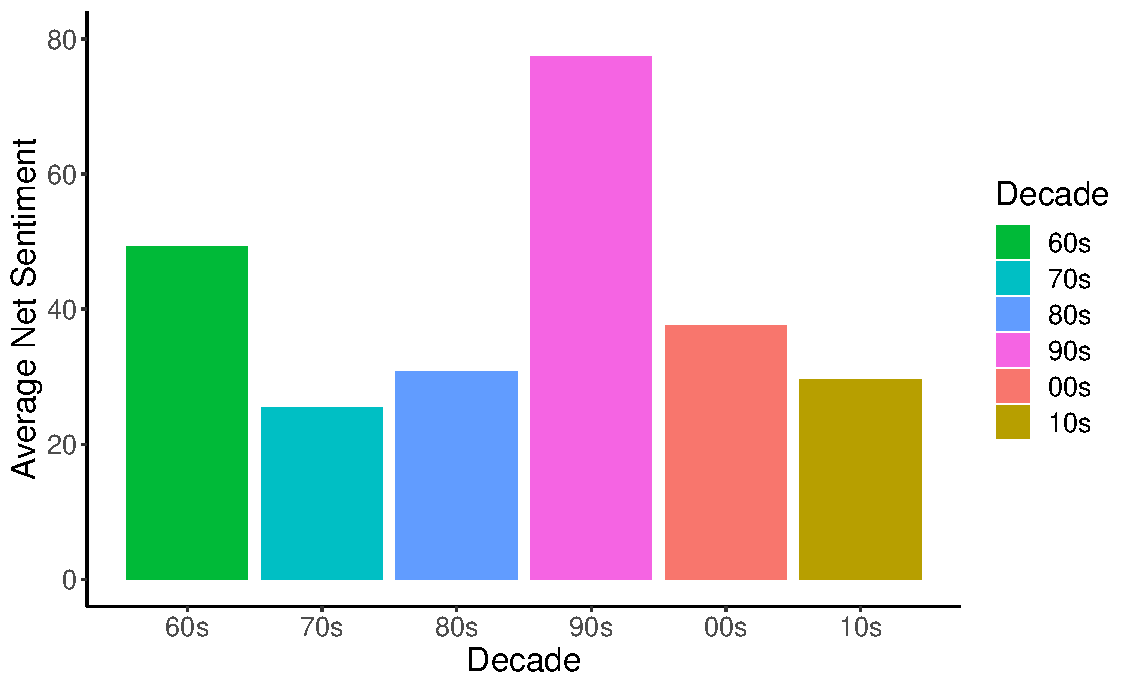
\includegraphics[scale=0.5]{Plots/graph_decade_mean_sentiment.pdf}
    \caption{Average net sentiment scores of the Grammy Albums of the Year, 1960--2019, by decade.}
    \label{fig:decade_sentiment}
\end{figure}


\FloatBarrier




\section*{And what about the losers?}


Albums that win the Grammy Award for Album of the Year are clearly outstanding, but it can be argued that merely being nominated is an honor in and of itself: albums that were nominated to the Grammy but did not win are also incredibly relevant. Thus, for every album in my original data set, I obtained the net sentiment of the albums that were also nominated that year but did not win (excluding live or comedy albums, albums whose lyrics where not in English, and classical music albums). This way I had the net sentiments of 56 albums that won and 216 albums that were only nominated. \\





\begin{figure}[h]
    \centering
    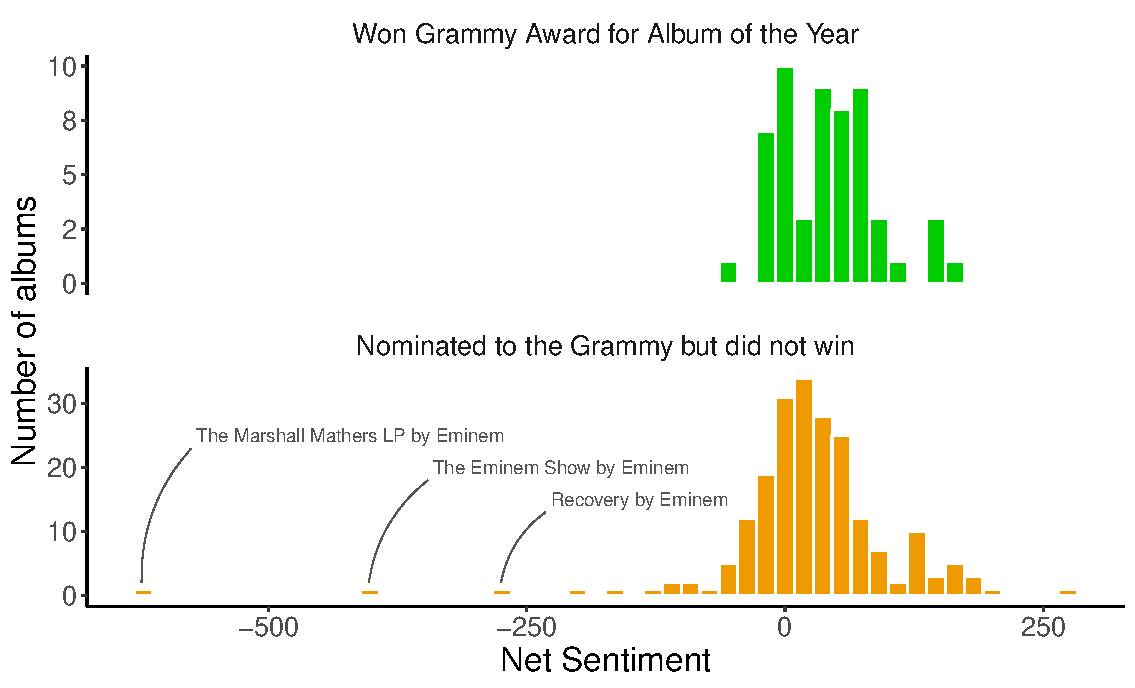
\includegraphics[scale=0.6]{Plots/graph_net_sentiment_histogram.pdf}
    \caption{Histograms of the net sentiments of the albums that won the Grammy Award for Album of the Year (green) and those that were nominated but did not win (orange), 1960--2019.}
    \label{fig:histogram}
\end{figure}




Winners and nominees tend to lie in the same range: the former's first and third quartiles are 7 and 71, respectively, versus -8 and 56 for the latter. Interestingly, both winners and nominees have the same \textit{interquartile range} (IQR, the difference between the third and first quartiles) of 64, although the nominees' IQR is shifted fifteen units to the left. This means that the nominees' net sentiments tend to be lower than the winners', which is corroborated in Figure \ref{fig:histogram}. This graph also shows that there are no winners with extreme sentiments, unlike some nominees. Of special interest are the three nominated albums with the lowest net sentiment. All correspond to the same artist, Eminem, one of the most renowned rappers of all time, whose music often deals with controversial and dark themes. \\






%\section*{HIStory: Past, Present, and Future}









\FloatBarrier

All in all, it seems that the only constant that can be observed is that Grammy Albums of the Year always seem to talk about love, whether the general tone is happier, as in the 1990s, or darker, as in the 2010s. This need not be particular to the Grammys: music in general often serves as an escape from reality in an age where, due to technology, we are constantly under a barrage of news and information. It offers a space in which artists express themselves and people from all around the globe can liken that music to their own actuality. Because of this, we will most likely never be able to completely grasp the complexities behind this subjective interchange. More so, maybe that is precisely the point of music. However, just by taking a data-driven glance at it, we can find all sorts of patterns and curiosities that, although falling short of giving us a full understanding, do offer a deeper look at it than what meets the eye.




\FloatBarrier
\nocite{*}
%\printbibliography
\bibliography{bibliography}




%Another way of attempting to predict the outcome of the Grammys is to estimate the probability that an album will win the Grammy based on its net sentiment, which can be done with a \textit{logistic regression}. This model relates the explanatory variable, in this case the net sentiment of an album, with the so-called \textit{log-odds} of the response variable. \\



%Suppose we have observed the net sentiment of a new album and want to determine its probability of winning the Grammy Award, $p$. Then the odds refer to the ratio $p / (1-p)$, the probability of winning divided by the probability of not winning. Odds are commonly used in gambling as a measure of payoff to stake, so that odds of 9 to 1 (as is commonly said) would mean that, for every dollar you bet, you get paid 9 dollars if you win. In that case, the probability of winning is $p=1/(1+9) = 0.1$, and so the odds would be 0.1/0.9. Finally, the log-odds are the logarithm of the odds. The model then assumes that, for an album that has probability $p$ of winning the Grammy Award,
%\begin{equation*}
%    \log \left( \frac{p}{1-p} \right) = a + b \times \text{Net sentiment},
%\end{equation*}
%where again $a$ and $b$ are unknown parameters to be estimated with the data of albums that both won and did not win the Grammy. \\

%and, with this information, found the estimates of the unknown parameters. However, the $b$ estimate ($\hat{b}= 0.003$), which is related to the percentage increase in the odds as a result of increasing the net sentiment, could again not be determined to be statistically different from zero. If anything, the model correctly assesses that albums with extremely negative net sentiments are very unlikely to win, as can be seen in Figure \ref{fig:logistic_regression}. However, albums with a net sentiment between 0 and 100 have less than a 0.25 estimated probability of winning the Grammy, even though more than half of past winners have net sentiments in that range! This is probably because albums that were nominated to the Grammy Award but did not win have similar net sentiments to those who actually won the award, and so the model cannot correctly single out the winners.


%\section*{Betting on the Grammys}


%Having obtained the net sentiment of every album that has won the Grammy Award for Album of the Year, it is possible to compute descriptive statistics of interest. For example, the average net sentiment of these albums is roughly 37, and half of them are between -39 and 123. In order to better quantify this, I obtained their \textit{probability density function} (pdf). This was done by a process called \textit{kernel smoothing}, which is very commonly used to estimate real-valued functions. I then used this information to estimate the probability of an album winning the Grammy Award based on its net sentiment as follows. \\







%The importance of knowing (at least approximately) the pdf is that it allows us to compute probabilities regarding the net sentiment of an album, given that it won the Grammy Award. That is, and using colors to better identify the factors under study, I obtained {\color{RoyalBlue} $P(\text{sentiment} \, | \, \text{Grammy})$}. Now imagine we could change the order and be able to compute probabilities of an album winning the Grammy Award, given its sentiment, {\color{Salmon} $P( \text{Grammy} \, | \, \text{sentiment} )$}. This can be done with the formula
%\begin{equation*}
%    {\color{Salmon} P( \text{Grammy} \, | \, \text{sentiment} )} = \frac{ {\color{RoyalBlue}  P(\text{sentiment} \, | \, \text{Grammy})} \times {\color{ForestGreen} P( \text{Grammy} )} }{ {\color{Brown} P( \text{sentiment} )} },
%\end{equation*}
%which is also known as \textit{Bayes' Theorem}. To summarise, by obtaining the net sentiments of albums that have won the Grammy Award we can effectively describe their behaviour, from a probabilistic point of view. Bayes' Theorem allows us to use this information to compute the probability of an album winning the Grammy Award, given that we know its net sentiment. Succinctly, we know {\color{RoyalBlue}blue} and want to obtain {\color{Salmon}red} = {\color{RoyalBlue}blue} $\times$ {\color{ForestGreen}green} / {\color{Brown}brown}. \\

%\begin{figure}[h]
%    \centering
%    \includegraphics[scale = 0.3]{graph_sentiment_posterior_density.pdf}
%    \caption{Plot of the probability density function of being awarded a Grammy given the sentiment, which is plotted in the $x$-axis.}
%    \label{fig:posterior_density}
%\end{figure}


%\begin{wrapfigure}{l}{0.55\textwidth}
%    \centering
%    \includegraphics[width=0.5\textwidth]{graph_densities_together.pdf}
%    \caption{The three probability density functions computed are shown.}
%    \label{fig:densities}
%\end{wrapfigure}


%The only caveat is that we know neither {\color{ForestGreen} $P(\text{Grammy})$} nor {\color{Brown} $P(\text{sentiment})$}. The former refers to our initial beliefs regarding an album's probabilities of winning the Grammy Award. I decided to pick {\color{ForestGreen} $P(\text{Grammy})$} so that it reflected no initial beliefs on the matter. This is to say that, prior to obtaining any information, there is no net sentiment that entails a greater chance of winning the Award. \\

%This is commonly done when one does not want that probability to heavily influence the rest of the analysis. \\

%I then used a Markov chain Monte Carlo (MCMC) method to obtain values of {\color{Salmon} $P( \text{Grammy} \, | \, \text{sentiment} )$}. These methods became popular in the 90s and are commonly used to solve problems in which values from a pdf are needed but can not be easily obtained. It was not necessary to estimate {\color{Brown} $P(\text{sentiment})$} because it is only a normalizing constant, and those have no effect when using this MCMC method, so that they can be omitted. \\

%Figure \ref{fig:densities} shows the resulting pdf of {\color{Salmon} $P( \text{Grammy} \, | \, \text{sentiment} )$}. With it, we can now estimate, given an album's net sentiment, its probability of winning the Grammy Award for Album of the Year. \\ 


%\begin{figure}[h]
%    \centering
%    \includegraphics[scale=0.6]{Plots/graph_posterior_density.pdf}
%    \caption{The pdf of {\color{Salmon} $P( \text{Grammy} \, | \, \text{sentiment} )$} is shown.}
%    \label{fig:densities}
%\end{figure}{}

%\newpage

%\begin{wrapfigure}{l}{0.4\textwidth}
%    \centering
%    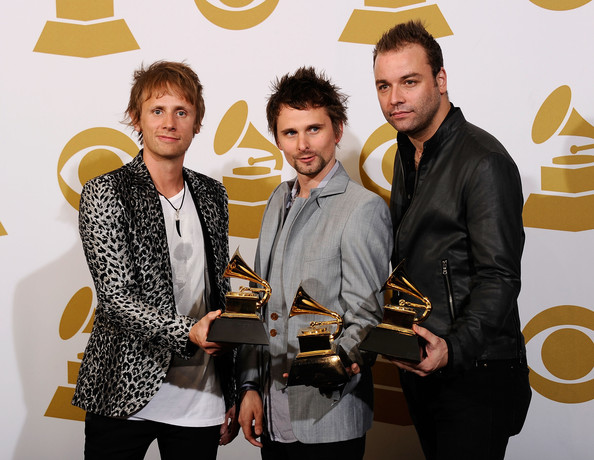
\includegraphics[width=0.37\textwidth]{Plots/MuseGrammys.jpg}
%    \caption*{Muse pose in the press room at The 53rd Grammy Awards after winning the Grammy Award for Best Rock Album for \textit{The Resistance} on February 2011. Source: \href{http://www.zimbio.com/photos/Dominic+Howard/Matt+Bellamy/53rd+Annual+GRAMMY+Awards+Press+Room/Olbz7K-nebK}{\bulurl{Zimbio}}.}
%\end{wrapfigure}

%As an example, I decided to estimate the probability that my favorite band, Muse, wins the next Grammy Award for Album of the Year. Muse are an English rock band formed in 1994, and they have already won two Grammy Awards for Best Rock Album (in 2011 for \textit{The Resistance} and again in 2016 for their latest work, \textit{Drones}). Now, Muse are expected to release a new album this year, with two singles, ``Dig Down'' and ``Thought Contagion'', already out. I obtained these songs' lyrics and computed their net sentiment, obtaining 2 and -5, respectively. Assuming that their new album will have a net sentiment between these values, I calculated their probability of winning the Grammy by numerically approximating the area below the {\color{Salmon}red} pdf of Figure \ref{fig:densities} between -5 and 2. I got an estimate of around 0.061, or roughly 6\%. This might just be Muse's lucky year. \\





\end{document}
